\documentclass[fontsize=12pt]{scrartcl}
\usepackage[ngerman]{babel}
\usepackage[utf8]{inputenc}
%\usepackage[latin1]{inputenc}
\usepackage{amsmath}
\usepackage{amstext}
\usepackage{amssymb}
\usepackage{stmaryrd}
\usepackage{verbatim}
\usepackage{mathrsfs}
\usepackage{extarrows}
\usepackage[arrow, matrix, curve]{xy}
\usepackage[centering,includeheadfoot,margin=2cm]{geometry}
\usepackage{gensymb}
\usepackage{graphicx}
\usepackage{framed}
\usepackage{xcolor}
\usepackage{float}
\usepackage{graphicx} 
\usepackage{sidecap}
\usepackage{blindtext,wrapfig}
\usepackage{epstopdf}
\usepackage{import}
\usepackage{fancyhdr}
\usepackage{fancybox}
\usepackage{graphicx}
\usepackage{caption}
\usepackage{subcaption}
\DeclareGraphicsRule{.tif}{png}{.png}{`convert #1 `basename #1 .tif`.png} 
\pagestyle{fancy}
\fancyhf{}
\fancyhead[R]{Physikalisches Praktikum 1}
\fancyhead[L]{Florentin Genth, Gentian Rrafshi}
\fancyfoot[R]{Seite \thepage}
\fancyfoot[L]{\today}

\begin{document}

\begin{minipage}{\textwidth}
\begin{center}\large
\title{K10d Abschwächung  von $\gamma$-Strahlung \\
		~\\
		~\\
		Assistent: \\
		 Sebastian Erfort \\
		 ~\\
		Datum Versuchsdurchführung: \\
		6.05.2015}

\author{bearbeitet von\\
		Gruppe 3-031: \\
		Florentin Genth Matrnr. 2952486 \\
		Gentian Rrafshi Matrnr. 2721617 }
\date{\today}

\maketitle

\end{center}
\end{minipage}

\newpage

\tableofcontents

\newpage
\noindent

\section{ Versuchsziel}

Bei diesem Versuch sollen jeweils der Schwächungskoeffizient und die Halbwertsdicke von Aluminium und Blei für die $\gamma$-Strahlung eines $^{60}$Co-Präparats bestimmt werden.

\section{ Grundlagen}

Grundlegend für den Versuch ist die Kenntnis darüber, dass es verschiedene Arten von \\
\glqq natürlichen\grqq~radioaktiven Strahlungen gibt.So ist eine Art von Strahlung die $\gamma$-Strahlung, welches im Grunde eine elektromagnetische 
Strahlung ist. Mit dieser Strahlung beschäftigen wir uns in diesem Versuch. \\
Weitere Arten von Strahlung sind die $\alpha$-Strahlung und die sogenannte $\beta^{-}$-Strahlung. Bei der $\alpha$-Strahlung löst sich aus dem Atomkern des radioaktiven Präparats ein 
Heliumkern und dieser wird abgestrahlt. Lösen sich aus dem Atomkern des radioaktiven Präparats nur Elektronen, so handelt es sich um eine $\beta^{-}$-Strahlung.$^{\cite{1}}$\\
~\\
Eine weitere Grundlage für diesen Versuch ist das Zerfallsgesetz und das Absorptionsgesetz, welche sich im Grunde ähneln.
So lautet das Zerfallsgesetz:
\begin{equation*}
n(t) = n_0\cdot e^{-\lambda \cdot t} 
\end{equation*}
Da alle drei Strahlungsarten sowohl Atome als auch Moleküle ionisieren, ist es möglich mit Hilfe eines Luftkondensators radioaktive Strahlung nachweisen.
Beim Eintreffen von Strahlungsteilchen auf Gasmoleküle oder Atome im Kondensator werden Elektronen frei.
Das elektrische Feld beschleunigt nun die Elektronen zur Anode hin. Dadurch entsteht ein geschlossener Stromkreis, welcher dann vom Zähler registriert wird.\\
~\\
Das Absorptionsgesetz beschreibt die absorbierende Wirkung eines Materials für $\gamma$-Strahlung. Sie lautet:
\begin{equation*}
Z = Z_0\cdot e^{-\alpha \cdot x} 
\end{equation*}
Wobei hier $n(t),n_0$ die Anzahl der zu Zeitpunkt $t$ bzw. $t=0$ noch vorhandenen Atomkerne und $Z,Z_0$ die Intensität der Strahlung ist.
$\lambda$ wird als Zerfallskonstante und $\alpha$ als Absorptionskoeffizient bzw. Abschwächungskoeffizienten bezeichnet.$^{\cite{2}}$ \\
~\\
Durch einsetzten von $n(t)=\frac{n_0}{2}$ bzw. $Z=\frac{Z_0}{2}$ erhält man durch umformen die Halbwertszeit $T_{1/2}$ und die Halbwertsdicke 
$x_{1/2}$, die wie folgt aussehen:$^{\cite{1}}$
\begin{align*}
T_{1/2} = \frac{\ln(2)}{\lambda} \\
~\\
x_{1/2} = \frac{\ln(2)}{\alpha}
\end{align*}
\newpage

\section{Versuchsaufbau und Durchführung}

\subsection{Benötigte Geräte}

\begin{figure}[h]
\centering
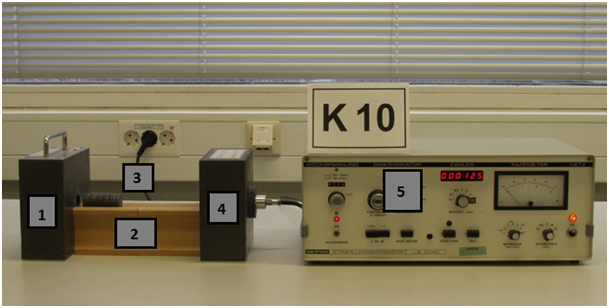
\includegraphics[scale=0.7]{Graphik/Versuchsaufbau}
\caption{Versuchsaufbau$^{\cite{A}}$}
\end{figure}

\begin{itemize}
\item[(1)] 	Bleiblock mit $^{60}$Co-Präparat
\item[(2)] 	Holzblock zur Auflage der Absorptionsklötze
\item[(3)] 	Verschieden dicke Absorptionsklötze aus Blei und Aluminium
\item[(4)] 	Bleiblock mit Geiger-Müller-Zähler
\item[(5)] 	Leybold-Zähler
\end{itemize}

\subsection{Bestimmung der Nullrate}
Die Bleiblöcke mit dem $^{60}$Co-Präparat (1) und dem Geiger-Müller-Zähler (4) werden längs nebeneinander gestellt, sodass die maximale Dicke an Blei 
zwischen Präparat und Zähler ist. Dadurch wird sichergestellt, dass so wenig Strahlung des Präparats wie möglich in den Zähler fällt, da man die Nullrate, also 
die Hintergrundstrahlung des Raums messen möchte. An dem Geiger-Müller-Zähler ist ein Leybold-Zähler (5) angeschlossen, der die vom Geiger-Müller-
Zähler ausgehenden Impulse zählt und pro eingestellter Zeiteinheit speichert. Nun stellt man ein, dass der Leybold-Zähler alle 60 Sekunden die Impulsrate 
speichert und lässt ihn 15 Minuten lang laufen. Die Werte werden notiert und der Mittelwert gebildet. \\
~\\
\subsection{Bestimmung der der Zählrate in Abhängigkeit der Dicke der Abschirmung}
Die Bleiblöcke mit dem $^{60}$Co-Präparat (1) und dem Geiger-Müller-Zähler (4) werden so aufgestellt, dass der Holzblock (3) genau dazwischen passt 
und der Geiger-Müller-Zähler bleibt am Leybold-Zähler (5) angeschlossen. Dieser Aufbau wird nicht mehr geändert, da die Strahlungsintensität auch vom 
Abstand abhängig ist und somit ein Umbau den Wert verändern könnte. Es werden nur Absorptionsblöcke (3) hinzugefügt oder weggenommen, da in 
Abhängigkeit der Dicke gemessen wird.\\
~\\
\textbf{Aluminium}\\
Es sind ein 2,5$\,\text{cm}$ langer und drei 5$\,\text{cm}$ lange Zylinder gegeben. Damit kann man Dicken von 0-17,5$\,\text{cm}$ in 2,5$\,\text{cm}$ 
Schritten erzeugen.\\
~\\
Zuerst werden die Impulsraten bei den ersten vier Dicken (0$\,\text{cm}$ bis 7,5$\,\text{cm}$) jeweils zwei Minuten lang gemessen. Dann werden die vier 
dicken Dicken (10$\,\text{cm}$ bis 17,5$\,\text{cm}$) jeweils fünf Minuten lang gemessen. Alle Messwerte werden dem Leybold-Zähler entnommen und 
notiert.\\
~\\
\textbf{Blei}\\
Es sind ein 0.5$\,\text{cm}$ langer und fünf 1$\,\text{cm}$ lange Zylinder gegeben. Damit kann man Dicken von 0-5,5$\,\text{cm}$ in 0,5$\,\text{cm}$ 
Schritten erzeugen. Wir betrachten die Dicken 0,5$\,\text{cm}$ bis 5$\,\text{cm}$.\\
~\\
Zuerst werden die Impulsraten bei den ersten sieben Dicken (0,5$\,\text{cm}$ bis 3,5$\,\text{cm}$) jeweils zwei Minuten lang gemessen. Dann werden die 
drei dicken Dicken (4$\,\text{cm}$ bis 5$\,\text{cm}$) jeweils fünf Minuten lang gemessen. Alle Messwerte werden dem Leybold-Zähler entnommen und 
notiert.
\newpage
\section{ Formeln}

\subsection{Formel zur Ermittlung des Mittelwerts:}

\begin{equation}
\bar{N_0}=\sum_{i=1}^n \frac{n_i}{i}
\end{equation}
\noindent
Hierbei ist $\bar{N}_0$ der Mittelwert, $i$ der Zeitpunkt der Messung und $n_i$ der Wert der jeweiligen Messung am Zeitpunkt $i$.

\subsection{Formeln für die effektive Zählrate:}
\begin{align}
Z_{\text{eff}} = Z – \bar{N_0}
\end{align}
\noindent
hierbei ist $Z$ die gemessene Zählrate und $\bar{N}$ der Mittelwert der Nullrate.

\subsection{Formeln für die Absorption von Gammastrahlen:}
\begin{align}
Z = Z_0\cdot e^{-\alpha \cdot x} 
\end{align}
\noindent
Hierbei ist $Z_0$ die vom Präparat ausgehende Zählrate, $Z$ ist die Zählrate, nachdem die Strahlung durch einen Metallblock der Dicke $x$ durchlaufen ist und $\alpha$ ist der Abschwächungskoeffizient. Dieser ist spezifisch für das Material der Blocks.

\subsection{Formel für die Berechnung der Halbwertsdicke $x_{1/2}$}
\begin{align}
x_{1/2} = \frac{\ln(2)}{\alpha}
\end{align}
\noindent
$\alpha$ ist der Abschwächungskoeffizient

\subsection{Formel für die Berechnung der noch nicht zerfallenen Kerne}
\begin{align}
n(t) = n_0\cdot e^{-\lambda \cdot t} 
\end{align}
\noindent
hierbei ist $n(t)$ die Zahl der noch nicht zerfallenen Kerne nach der Zeit $t,~n_0$ die Zahl der zu Beginn vorhandenen Kerne und $\lambda$ die Präparat spezifische Zerfallskonstante (der Kehrwert der mittleren Lebensdauer)

\subsection{Formel für die Berechnung der Zerfallskonstante}
\begin{align}
T_{1/2} = \frac{\ln(2)}{\lambda}
\end{align}
\noindent
hierbei ist $T_{1/2}$ die Halbwertszeit.

\subsection{Formel für die Berechnung der Aktivität}
\begin{align}
A= A_0 \cdot e^{-\lambda\cdot t}
\end{align}
\noindent
Wobei hier $A$ die Aktivität und $A_0$ die Aktivität am 1.1.2009 ist vom Cobalt-Präparat.

\section{ Messwerte}
\begin{figure}[h]
\centering
\caption{Messwerte}
\begin{tabular}{|c|c|} \hline
Zeit [min] &	Nulleffekt $N_0$ [Impulse/min] \\ \hline
1	&82 \\ \hline
2	&87 \\ \hline
3	&78 \\ \hline
4	&92 \\ \hline
5	&96 \\ \hline
6	&93 \\ \hline
7	&104 \\ \hline
8	&113 \\ \hline
9	&99 \\ \hline
10	&97 \\ \hline
11		&94 \\ \hline
12	&116 \\ \hline
13	&122 \\ \hline
14	&80 \\ \hline
15	&89 \\ \hline
\end{tabular} \\
\end{figure} 
\noindent
\newpage
\begin{figure}[h!]
\begin{minipage}{0.5\textwidth}
\centering
\vspace{-120pt}
\caption{Messwerte  für Aluminium}
\begin{tabular}{|c|c|c|} \hline
Zeit [min]	&	$Z$ [Impulse/min]	&	Abstand [cm] \\ \hline
1			&820		&0,00 \\ \hline
2			&869		&0,00 \\ \hline
3			&589		&2,50 \\ \hline
4			&610		&2,50 \\ \hline
5			&418		&5,00 \\ \hline
6			&436		&5,00 \\ \hline
7			&324		&7,50 \\ \hline
8			&340		&7,50 \\ \hline
9			&248		&10,00 \\ \hline
10		&239		&10,00 \\ \hline
11			&241		&10,00 \\ \hline
12		&253		&10,00 \\ \hline
13		&217		&10,00 \\ \hline
14		&209		&12,50 \\ \hline
15		&215		&12,50 \\ \hline
16		&182		&12,50 \\ \hline
17		&193		&12,50 \\ \hline
18		&209		&12,50 \\ \hline
19		&143		&15,00 \\ \hline
20		&167		&15,00 \\ \hline
21		&172		&15,00 \\ \hline
22		&171		&15,00 \\ \hline
23		&182		&15,00 \\ \hline
24		&132		&17,50 \\ \hline
25		&160		&17,50 \\ \hline
26		&125		&17,50 \\ \hline
27		&160		&17,50 \\ \hline
28		&148		&17,50 \\ \hline
\end{tabular} \\
\end{minipage}
\begin{minipage}{0.5\textwidth}
\centering
\caption{Messwerte  für Blei}
\begin{tabular}{|c|c|c|} \hline
Zeit [min]			&	$Z$ [Impulse/min]	&Abstand [cm] \\ \hline
1						&830		&0,00  \\ \hline
2						&865		&0,00  \\ \hline
3						&699		&0,50 \\ \hline
4						&647		&0,50 \\ \hline
5						&510		&1,00 \\ \hline
6						&486		&1,00 \\ \hline
7						&391		&1,50 \\ \hline
8						&394		&1,50 \\ \hline
9						&337		&2,00 \\ \hline
10					&348		&2,00 \\ \hline
11						&274		&2,50 \\ \hline
12					&266		&2,50 \\ \hline
13					&226		&3,00 \\ \hline
14					&236		&3,00 \\ \hline
15					&186		&3,50 \\ \hline
16					&190		&3,50 \\ \hline
17					&143		&4,00 \\ \hline
18					&153		&4,00 \\ \hline
19					&139		&4,00 \\ \hline
20					&151		&4,00 \\ \hline
21					&166		&4,00 \\ \hline
22					&129		&4,50 \\ \hline
23					&141		&4,50 \\ \hline
24					&144		&4,50 \\ \hline
25					&146		&4,50 \\ \hline
26					&146		&4,50 \\ \hline
27					&119		&5,00 \\ \hline
28					&133		&5,00 \\ \hline
29					&141		&5,00 \\ \hline
30					&137		&5,00 \\ \hline
31					&129		&5,00 \\ \hline
32					&109		&5,50 \\ \hline
33					&128		&5,50 \\ \hline
34					&108		&5,50 \\ \hline
35					&101		&5,50 \\ \hline
36					&95			&5,50 \\ \hline
\end{tabular} \\
\end{minipage}
\end{figure}


\section{ Auswertung}

\subsection{Ermittlung der durchschnittlichen Messwerte}

Zur Berechnung unserer durchschnittlichen Werte wird die übliche Formel für die Berechnung des Mittelwerts verwendet. Aufgrund der Übersichtlichkeit wird hier nur das Ergebnis angegeben für die Nullrate:\\
\begin{equation*}
\bar{N_0}=\sum_{i=1}^k \frac{n_i}{i} = \sum_{i=1}^{15} \frac{n_i}{i} = 96,64\,\frac{\text{Impulse}}{\text{min}}
\end{equation*}
\noindent
Und hier wird der durchschnittlicher Messwert für die dicke von $2,50$\,cm bei Aluminium ausführlicher errechnet und am Ende der Auswertung in einer Tabelle angegeben:
\begin{equation*}
\bar{Z}_{\text{2,5}}=\sum_{i=1}^k \frac{n_i}{i} = \sum_{i=1}^{2} \frac{Z_i}{i} = \frac{820\,\frac{\text{Impulse}}{\text{min}}+869\,\frac{\text{Impulse}}{\text{min}}}{2} = 845\,\,\frac{\text{Impulse}}{\text{min}}
\end{equation*}
\subsection{Berechnung der effektiven Zählrate}
Zur Bestimmung der effektiven Zählrate wird hier eine Beispielrechnung für Aluminium zur Zeiteinheit $t=1$\,min gezeigt. Am Ende der Auswertung stehen alle anderen errechneten Werte in einer Tabelle aufgeführt.
\begin{align*}
Z_{\text{eff}} = Z – \bar{N}= 854\,\frac{\text{Impulse}}{\text{min}}-96,64\,\frac{\text{Impulse}}{\text{min}} =747,86\,\frac{\text{Impulse}}{\text{min}}
\end{align*}
\noindent
\subsection{Bestimmung von $\alpha$}
Das Plotprogramm Qtiplot fittet an unsere Messwerte Geraden mit folgenden $\alpha$, welches hier ebenfalls der Abschwächungskoeffizient ist.
\begin{itemize}
\centering
\item[\textbf{Aluminium}] $\alpha=0,16\,\frac{1}{\text{cm}}$
\item[\textbf{Blei}] $\alpha=0,56\,\frac{1}{\text{cm}}$
\end{itemize}

\subsection{Berechnung der Halbwertsdicke $x_{1/2}$}

Ein Versuchsziel ist es, die Halbwertsdicke für Aluminium und Blei zu bestimmen. Dafür benötigen wir lediglich die Formel (4), die durch einsetzen von $Z=\frac{Z_0}{2}$ in (3) und Umformung erfolgt:
\begin{align*}
x_{1/2~\text{Alu}} = \frac{\ln(2)}{\alpha}= \frac{\ln(2)}{0,16\,\frac{1}{\text{cm}}}=4,36\,\text{cm}\\
~\\
x_{1/2~\text{Blei}} = \frac{\ln(2)}{\alpha}= \frac{\ln(2)}{0,56\,\frac{1}{\text{cm}}}=1,23\,\text{cm} 
\end{align*}

\newpage
\subsection{Berechnung der Aktivität des  $^{60}$Co-Präparats}

Zu aller erst wurden folgende Werte vom Präparat abgelesen:
\begin{itemize}
\item[1.]	Zeit an dem die Aktivität ausgerechnet wird  13.5.2015
\item[2.]	Die Halbwertszeit beträgt $T_{1/2}=5,272$\,Jahre
\item[3.]	Aktivität am 1.1.2009 $A=886$\,kBq
\end{itemize}
Der Zeitunterschied vom 1.1.2009 bis zum 13.5.2015 sind $3345840\,\text{min}$.\\
Für $\lambda$ folgt mit Formel (6):
\begin{equation*}
\lambda  = \frac{\ln(2)}{T_{1/2}} =  \frac{\ln(2)}{2770963\,\text{min}}= 0,0000002501\,\frac{1}{\text{min}}
\end{equation*}
und dadurch ergibt sich für die Aktivität:
\begin{align*}
A = {\lambda}\cdot \tilde{n} = {\lambda}\cdot n_0 \cdot e^{-\lambda\cdot t}\quad\text{und}\quad
n_0 =\frac{A_0}{\lambda}
\end{align*}
Woraus sich Formel (7) ergibt:
\begin{align*}
A= A_0 \cdot e^{-\lambda\cdot t}=886\,\text{kBq}\cdot  e^{- 0,0000002501\,\frac{1}{\text{min}} \cdot 3345840\,\text{min}}=886\,\text{kBq}\cdot 0,43 = 383,66\,\text{kBq}
\end{align*}
\noindent

\subsection{Tabelle für die Auswertungen}
\begin{figure}[h!]
\begin{minipage}{0.5\textwidth}
\centering
\caption{Messwerte  für Aluminium}
\begin{tabular}{|c|c|} \hline
$Z_{\text{eff}}$ [Impulse/min]	&	Abstand [cm] \\ \hline
747,86	&0,00 \\ \hline
502,86	&2,50\\ \hline
330,36	&5,00\\ \hline
235,36	&7,50\\ \hline
142,96	&10,00\\ \hline
112,36	&12,50\\ \hline
65,86	&15,00\\ \hline
43,36	&17,50\\ \hline
\end{tabular} \\
\end{minipage}
\begin{minipage}{0.5\textwidth}
\centering
\caption{Messwerte  für Blei}
\begin{tabular}{|c|c|c|} \hline
$Z_{\text{eff}}$ [Impulse/min]	&Abstand [cm] \\ \hline
750,86	&0,00 \\ \hline
576,36	&0,50 \\ \hline
401,36	&1,00 \\ \hline
295,86	&1,50 \\ \hline
245,86	&2,00 \\ \hline
173,36	&2,50 \\ \hline
134,36	&3,00 \\ \hline
91,36	&3,50 \\ \hline
53,76	&4,00 \\ \hline
40,86	&4,50 \\ \hline
27,36	&5,00 \\ \hline
11,56	&5,50 \\ \hline
\end{tabular} \\
\end{minipage}
\end{figure}
\noindent
Die folgenden Diagramme bilden die Zählrate in Abhängigkeit von der Abschirmdicke, wobei die $y$-Achse logarithmiert ist. Auch die Fehlerbalken für die Zählrate und Ausgleichsgeraden wurden schon hinzugefügt und werden in den jeweiligen Abschnitten bei der Fehlerrechnung ausführlich erklärt bzw. berechnet. 
\begin{figure}[h!]
\centering
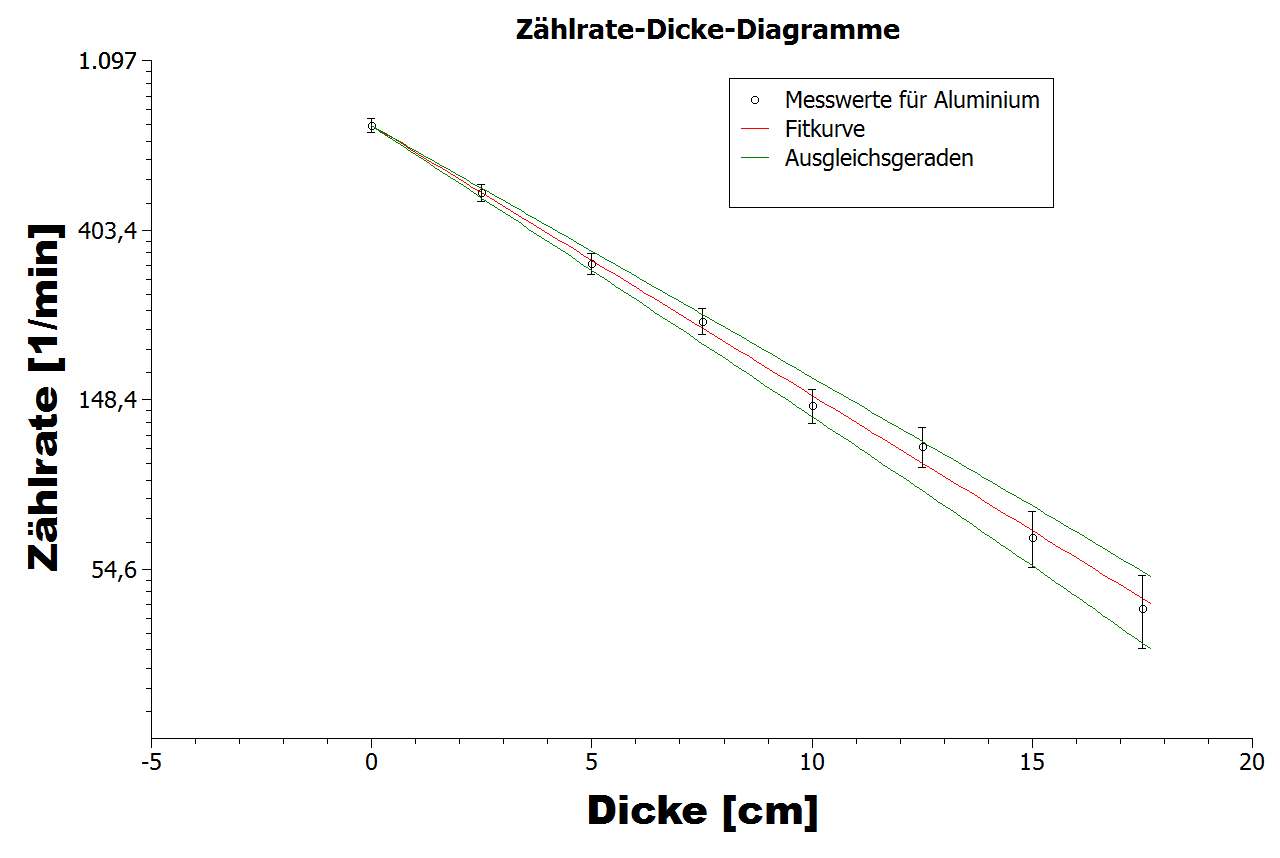
\includegraphics[scale=0.4]{Graphik/Alu}
\caption{Zählrate-Dicke-Diagramm für Aluminium}
\end{figure}
\begin{figure}[h!]
\centering
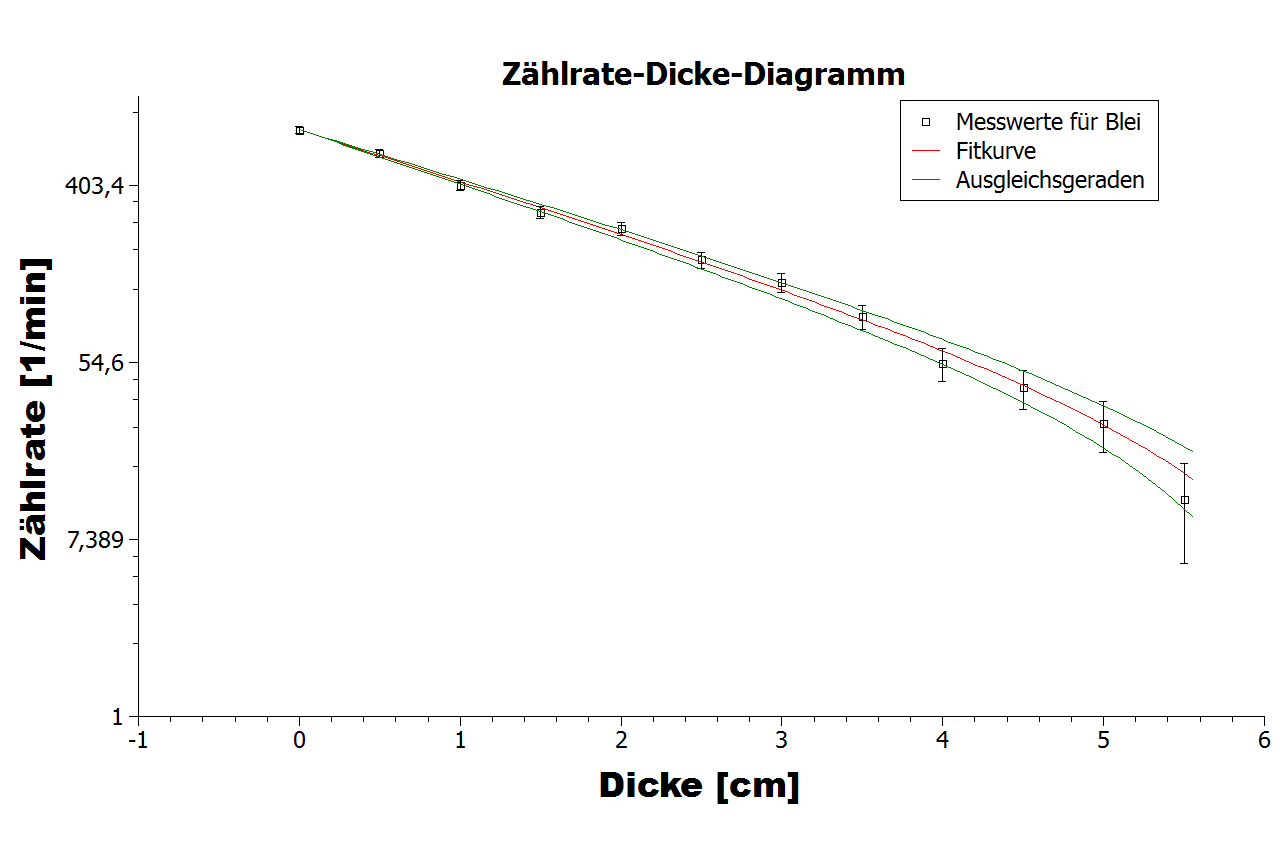
\includegraphics[scale=0.4]{Graphik/Blei}
\caption{Zählrate-Dicke-Diagramm für Blei}
\end{figure}
\newpage
\section{Fehlerquellen und Fehlerrechnung}

\subsection{Fehlerquellen}
Der radioaktive Zerfall von Atomkernen ist ein Zufallsprozess, dies erklärt die großen Schwankungen bei den Messwerten. Eine weitere Fehlerquelle sind die Messgeräte. Diese haben Toleranzbereiche, die eine Ungenauigkeit bei unseren Messwerten herbeiführen.

\subsection{Fehlerrechnung}

\subsubsection{Fehler bei der Nullrate}
Da die Zahl der Zerfälle Poisson-verteilt ist, gilt folgende Formel für unseren Fehler bei der Nullrate:
\begin{align*}
\Delta n_Z &= \sqrt{n_z}=\sqrt{\sum_{i=1}^k {n_i}} =\sqrt{ \sum_{i=1}^{15} {n_i}} =\sqrt{1442,00} = 37,97 \\
\Delta \bar{N_0} &= \frac{\Delta n_Z}{t} = \frac{\sqrt{ \sum_{i=1}^{15} {n_i}}}{15\,\text{min}} = \frac{\sqrt{1442,00}}{15\,\text{min}} = 2,53\,\frac{1}{\text{min}}
\end{align*}
Zu Bedenken ist hier, das die Zahl der Zerfälle $n_z$ Einheitslos ist, bzw. einfach nur ein Impuls ist.
Daher erhalten wir für die Nullrate folgendes Ergebnis:
\begin{equation*}
\bar{N}_0= 96,64\,\frac{\text{Impulse}}{\text{min}}~\pm2,53\,\frac{\text{Impulse}}{\text{min}}
\end{equation*}

\subsubsection{Fehler bei der effektiven Zählrate}
Durch Ausnutzen von:
\begin{equation*}
n_z = Z \cdot t \Longleftrightarrow Z= \frac{n_z}{t}
\end{equation*}
erhalten wir
\begin{equation*}
\Delta Z_{\text{eff}}= \vert \frac{\partial Z}{\partial n_z}\vert \cdot \Delta n_z =\frac{ \sqrt{n_z} }{t} = \sqrt{\frac{Z}{t}}
\end{equation*}
Für die effektive Zählrate gilt jedoch:
\begin{align*}
\Delta Z_{\text{eff}} &=\frac{\partial Z_{\text{eff}}}{\partial Z} Z + \frac{\partial Z_{\text{eff}}}{\partial N}\bar{N_0} \\
&=\Delta Z + \Delta \bar{N_0} \\
&= \sqrt{\frac{Z}{t}} + \Delta \bar{N_0} 
\end{align*}
Eine Beispielrechnung erfolgt hier für Aluminium bei einer Dicke von $2,5$\,cm:
\begin{equation*}
\Delta Z_{\text{eff}} = \sqrt{\frac{Z}{t}} + \Delta \bar{N_0} = \sqrt{747,86}\,\frac{\text{Impulse}}{\text{min}} + \Delta \bar{2,53}\,\frac{\text{Impulse}}{\text{min}} =24,95 \,\frac{\text{Impulse}}{\text{min}}
\end{equation*}
\noindent
In folgender Tabelle sind unsere restlichen Ergebnisse für die effektive Zählrate:
\begin{figure}[h!]
\centering
\caption{Ergebnisse  für Aluminium}
\begin{tabular}{|c|c|c|} \hline
$Z_{\text{eff}}$ [Impulse/min] & $\Delta Z_{\text{eff}}$ [Impulse/min]	&Abstand [cm] \\ \hline
747,86	&29,88	&0,00\\ \hline
502,86	&24,95	&2,50\\ \hline
330,36	&20,71	&5,00\\ \hline
235,36	&17,87	&7,50\\ \hline
142,96	&14,49	&10,00\\ \hline
112,36	&13,13	&12,50\\ \hline
65,86	&10,65	&15,00\\ \hline
43,36	&9,11		&17,50\\ \hline
\end{tabular} \\
\end{figure}
\begin{figure}[h!]
\centering
\caption{Ergebnisse  für Blei}
\begin{tabular}{|c|c|c|} \hline
$Z_{\text{eff}}$ [Impulse/min] & $\Delta Z_{\text{eff}}$ [Impulse/min]	&Abstand [cm] \\ \hline
750,86	&29,93	&0,00\\ \hline
576,36	&26,54	&0,50\\ \hline
401,36	&22,56	&1,00\\ \hline
295,86	&19,73	&1,50\\ \hline
245,86	&18,21	&2,00\\ \hline
173,36	&15,70	&2,50\\ \hline
134,36	&14,12	&3,00\\ \hline
91,36	&12,09	&3,50\\ \hline
53,76	&9,86	&4,00\\ \hline
40,86	&8,92	&4,50\\ \hline
27,36	&7,76	&5,00\\ \hline
11,56	&5,93	&5,50\\ \hline
\end{tabular} \\
\end{figure}

\subsubsection{Fehler beim Abschwächungskoeffizient}

Das Programm QtiPlot gibt uns automatisch beim Fitten auch die Fehler für $\alpha$ an.
Wir erhalten für Aluminium:
\begin{itemize}
\item[1)] $\alpha_{max}=0,17\,\frac{1}{\text{cm}}$
\item[2)] $\alpha_{min}=0,15\,\frac{1}{\text{cm}}$
\end{itemize}
und für Blei:
\begin{itemize}
\item[1)] $\alpha_{max}=0,59\,\frac{1}{\text{cm}}$
\item[2)] $\alpha_{min}=0,54\,\frac{1}{\text{cm}}$
\end{itemize}
\newpage
\noindent
Daraus ergibt sich $\Delta \alpha$ wie folgt:
\begin{equation*}
\Delta \alpha = \max\{ \vert \alpha - \alpha_{max}\vert ; \vert \alpha - \alpha_{min}\vert \}
\end{equation*}
Wodurch wir dann als $\Delta \alpha$ folgendes herausbekommen:
\begin{align*}
\Delta \alpha_{\text{Alu}} &= \max\{ \vert 0,16\,\frac{1}{\text{cm}} - 0,17\,\frac{1}{\text{cm}}\vert ; \vert 0,16\,\frac{1}{\text{cm}} - 0,15\,\frac{1}{\text{cm}}\vert \} = 0,01\,\frac{1}{\text{cm}} \\
~\\
\Delta \alpha_{\text{Blei}} &= \max\{ \vert 0,56\,\frac{1}{\text{cm}} - 0,59\,\frac{1}{\text{cm}}\vert ; \vert 0,56\,\frac{1}{\text{cm}} - 0,54\,\frac{1}{\text{cm}}\vert \} = 0,03\,\frac{1}{\text{cm}} 
\end{align*}
\subsubsection{Berechnung der Halbwertsdicke $\Delta x_{1/2}$}

Mit Hilfe von Formel (4)  können wir den Fehler $\Delta x_{1/2}$ wie folgt berechnen:
\begin{align*}
\Delta x_{1/2} = \vert \frac{\partial x_{1/2}}{\partial \alpha} \vert \cdot \Delta \alpha = \vert-\frac{\ln(2)}{\alpha^2} \vert \cdot \Delta\alpha
\end{align*}
Dadurch ergibt sich dann für unsere Messwerte:
\begin{align*}
\Delta x_{1/2~Alu}  &= \vert-\frac{\ln(2)}{\alpha^2} \vert \cdot \Delta\alpha = \frac{\ln(2)}{0,16\,\frac{1}{\text{cm}^2}} \cdot 0,01\,\frac{1}{\text{cm}} \\
 & = 0,27\,\frac{1}{\text{cm}} \\
 ~\\
 \Delta x_{1/2~Blei}  &= \vert-\frac{\ln(2)}{\alpha^2} \vert \cdot \Delta\alpha = \frac{\ln(2)}{0,56\,\frac{1}{\text{cm}^2}} \cdot 0,03\,\frac{1}{\text{cm}} \\
 & = 0,07\,\frac{1}{\text{cm}}
\end{align*}
Um etwas Übersichtlichkeit zu schaffen, wird die nachfolgende Tabelle alles wichtige für den Abschwächungskoeffizienten und der Halbwertsdicke aufgeführt:
\begin{figure}[h!]
\centering
\caption{Fehler für $\alpha$ und $x_{1/2}$}
\begin{tabular}{|ll|c|c|} \hline
 && Aluminium	& Blei \\ \hline
Abschwächungskoeffizient& $\alpha\pm\Delta\alpha\,[\frac{1}{\text{cm}}]$ & $0,16\pm 0,01$ & $0,56\pm 0,03$ \\ \hline
Halbwertsdicke& $ x_{1/2}\pm\Delta x_{1/2}\,[\text{cm}]$ &$ 4,36 \pm 0,27$ & $1,23\pm 0,07$ \\ \hline
\end{tabular}
\end{figure}



\newpage

\section{Zusammenfassung}
Ziel des Versuchs war es den Abschwächungskoeffizient und die Halbwertsdicke von Aluminium und Blei für die $\gamma$-Strahlung eines $^{60}$Co-
Präparats zu bestimmen. Es stellt sich bei uns für den Abschwächungskoeffizienten heraus, dass der von Blei um einiges höher ist.
~\\
Desweiteren ist die Halbwertsdicke von Blei um einiges kleiner als die von Aluminium, d.h. man braucht eine um einiges dünnere Schicht Blei um $\gamma$-Strahlung abzuschirmen. Dies passt mit unseren Ergebnissen über den Abschwächungskoeffizienten überein, da ein hoher Abschwächungskoeffizient eben eine kleinere Halbwertsdicke mit sich zieht.\\
~\\
Vergleicht man unsere Messwerte mit den errechneten Halbwertsdicken, sind diese zudem recht nah beieinander. \\
~\\
Generell sind auch unsere Fehler nicht groß. Prozentual sind wir mit unseren Fehlern beim Abschwächungskoeffizienten und der Halbwertsdicke bei $\approx 6\%$.
\newpage
         
\section{Literaturverzeichnis}
 \renewcommand\refname{~}
 \vspace{-25pt}

\begin{thebibliography}{xxx}
\bibitem{1}		\glqq \textit{K10 Abschwächung  von $\gamma$-Strahlung}\grqq, in\\
						\textit{http:www3.physik.uni-stuttgart.de/studium/praktika/ap/}, unter\\
						\textit{http://www3.physik.uni-stuttgart.de/studium/praktika/ap/pdf\_dateien/K10.pdf}; \\
						abgerufen am 11.05.2015
\bibitem{2}		Gerthsen Physik, Springer, 24. Auflage 2010 S. 179, 945
\bibitem{A}		Graphik aus \glqq \textit{K10 Abschwächung  von $\gamma$-Strahlung}\grqq, in\\
						\textit{http://www3.physik.uni-stuttgart.de/studium/praktika/ap/}, unter \\
						\textit{http://www3.physik.uni-stuttgart.de/studium/praktika/ap/bilder/?Name=K10.jpg}; \\
						abgerufen am 11.05.2015


\end{thebibliography}

\section{Anhang}


\end{document}